\chapter{Python scripts}
\label{Cha: Bijlage_F}

\section{wielassen.}
\label{Se: bijlage_F wielassen}
\begin{figure}[H]
    \centering
    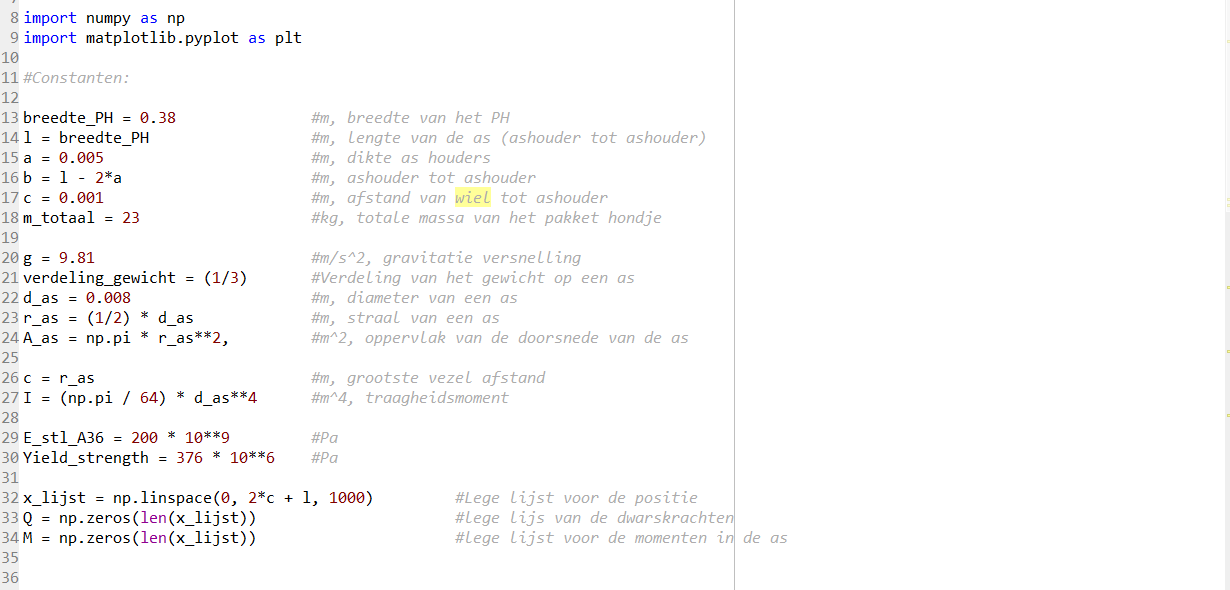
\includegraphics[width = 120mm]{06_bijlage_F/As_script/Doorbuiging_as_constanten.PNG}
    \caption{Python script, doorbuiging assen, constanten.}
    \label{fig:python_d.a._constanten}
\end{figure}

\vspace{\baselineskip}

\begin{figure}[H]
    \centering
    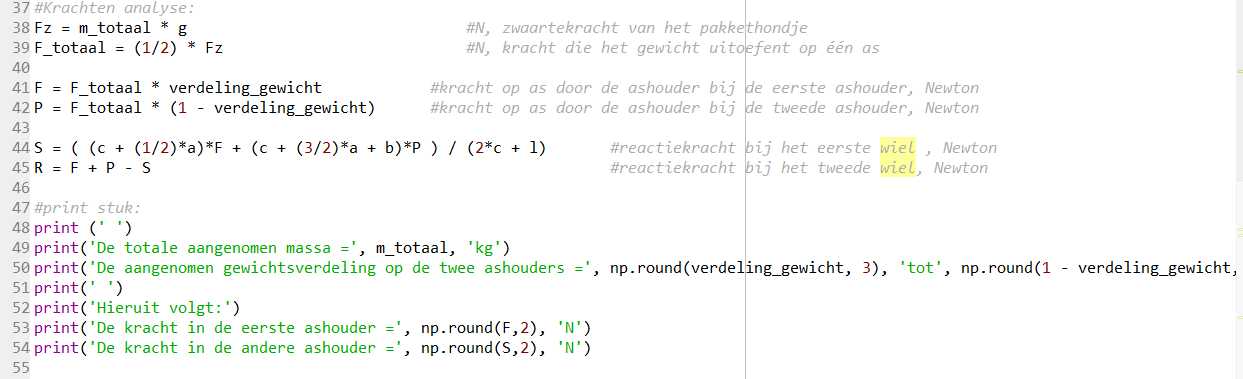
\includegraphics[width = 120mm]{06_bijlage_F/As_script/Doorbuiging_as_krachten_analyse.PNG}
    \caption{Python script, doorbuiging assen, krachten analyse.}
    \label{fig:python_d.a._krachtenanalyse}
\end{figure}

\vspace{\baselineskip}

\begin{figure}[H]
    \centering
    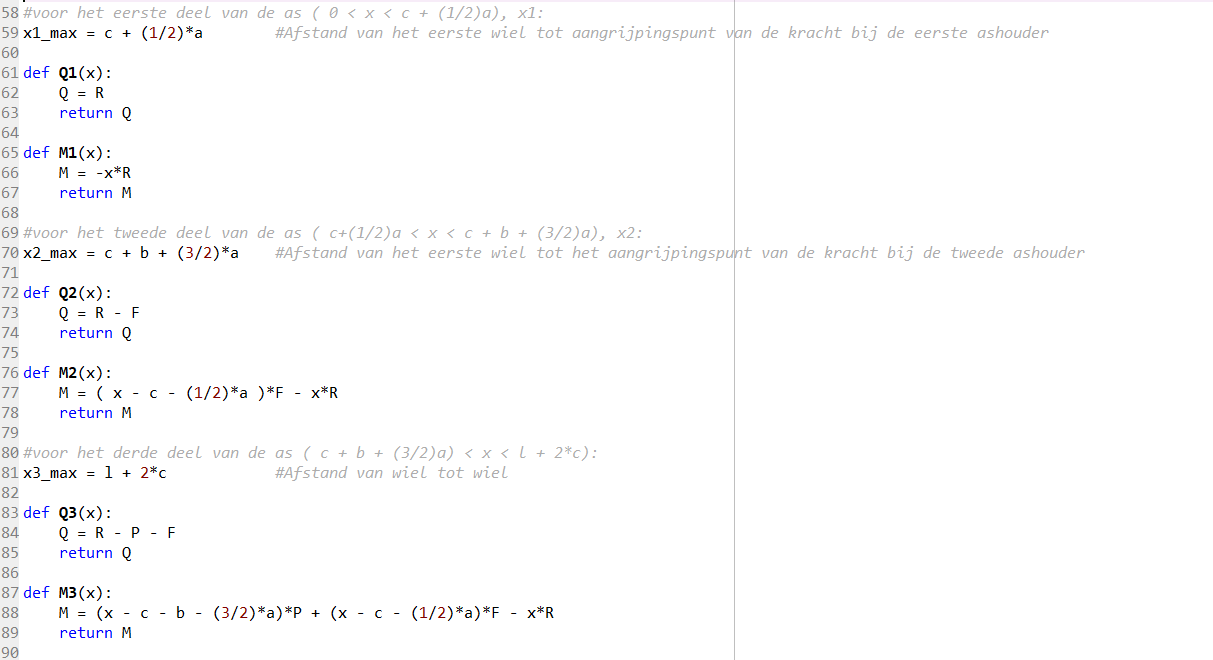
\includegraphics[width = 120mm]{06_bijlage_F/As_script/Doorbuiging_as_functies.PNG}
    \caption{Python script, doorbuiging assen, functies van dwarskrachten en momenten.}
    \label{fig:python_d.a._functies}
\end{figure}

\vspace{\baselineskip}

\begin{figure}[H]
    \centering
    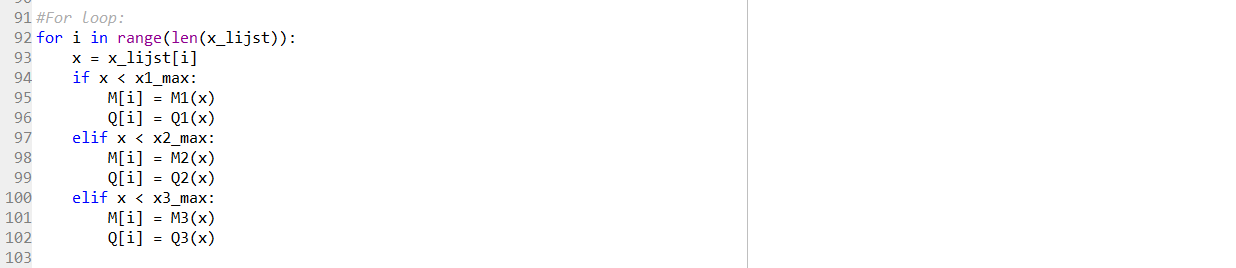
\includegraphics[width = 120mm]{06_bijlage_F/As_script/Doorbuiging_as_forloop.PNG}
    \caption{Python script, doorbuiging assen, for-loop.}
    \label{fig:python_d.a._forloop}
\end{figure}

\vspace{\baselineskip}

\begin{figure}[H]
    \centering
    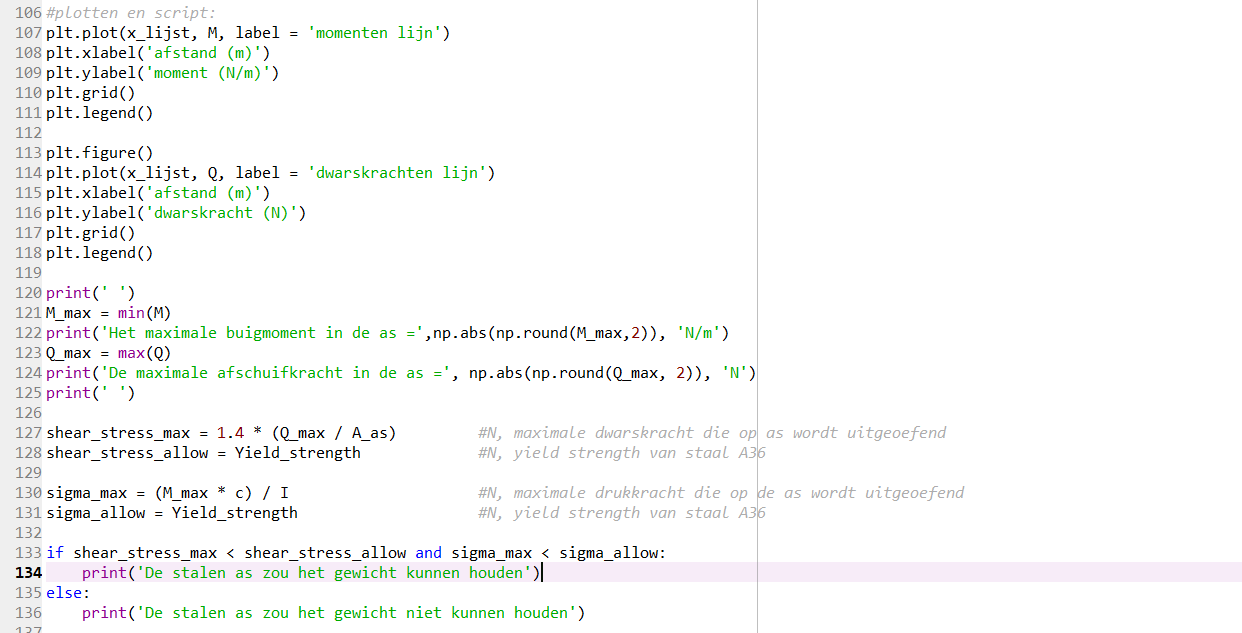
\includegraphics[width = 120mm]{06_bijlage_F/As_script/Doorbuiging_as_plottenprinten.PNG}
    \caption{Python script, doorbuiging assen, plots en print waarden.}
    \label{fig:python_d.a._plotsenprints}
\end{figure}
\vspace{\baselineskip}

\section{Schaarliften}
\label{se: bijlage_F schaarliften}
\vspace{\baselineskip}

\begin{figure}[H]
    \centering
    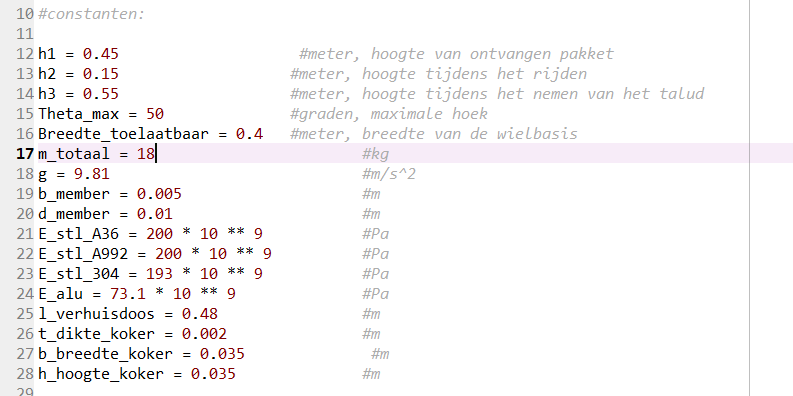
\includegraphics[width = 120mm]{04_conceptdimensionering/Constanten_schaarlift.PNG}
    \caption{Python script, schaarliften.}
    \label{fig:schaarliften_constanten}
\end{figure}
\vspace{\baselineskip}

\begin{figure}[H]
    \centering
    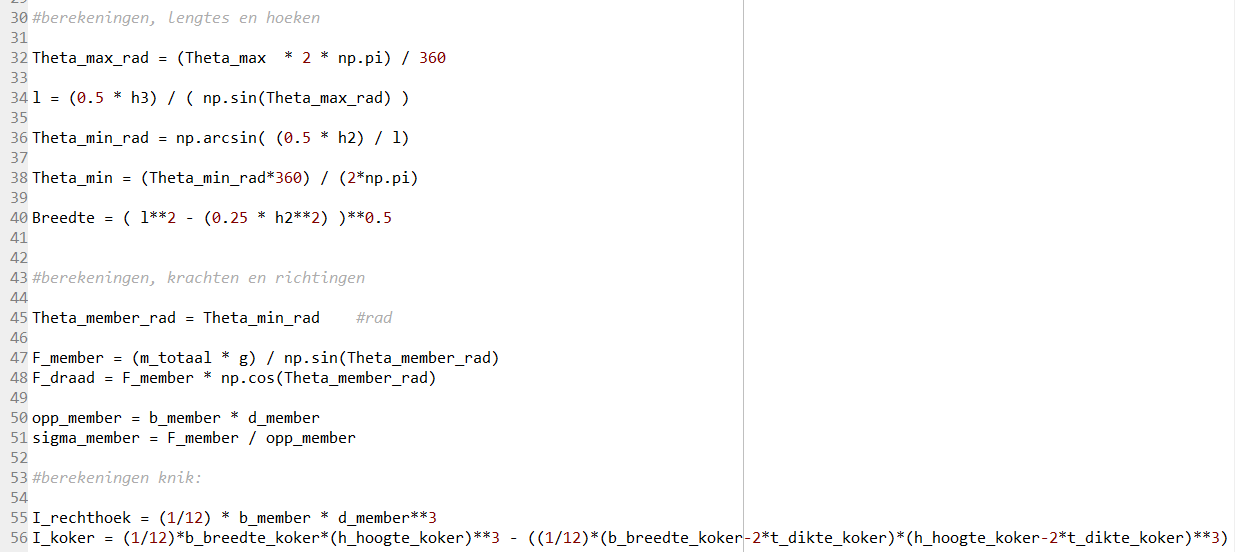
\includegraphics[width = 120mm]{06_bijlage_F/Schaarlift_script/berekeningen_schaarlift.PNG}
    \caption{Python script, schaarliften.}
    \label{fig:schaarliften_berekeningen}
\end{figure}
\vspace{\baselineskip}

\begin{figure}[H]
    \centering
    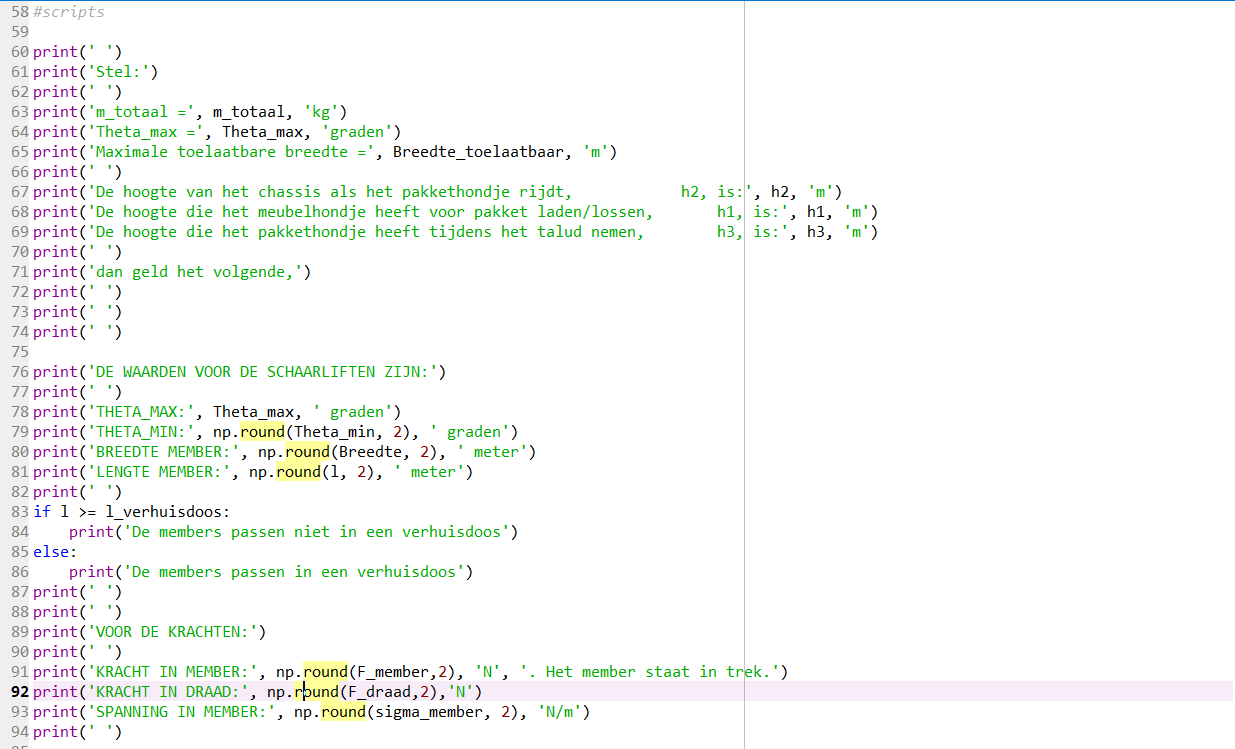
\includegraphics[width = 120mm]{06_bijlage_F/Schaarlift_script/prints1_schaarlift.PNG}
    \caption{Python script, schaarliften.}
    \label{fig:schaarliften_sript1}
\end{figure}
\vspace{\baselineskip}

\begin{figure}[H]
    \centering
    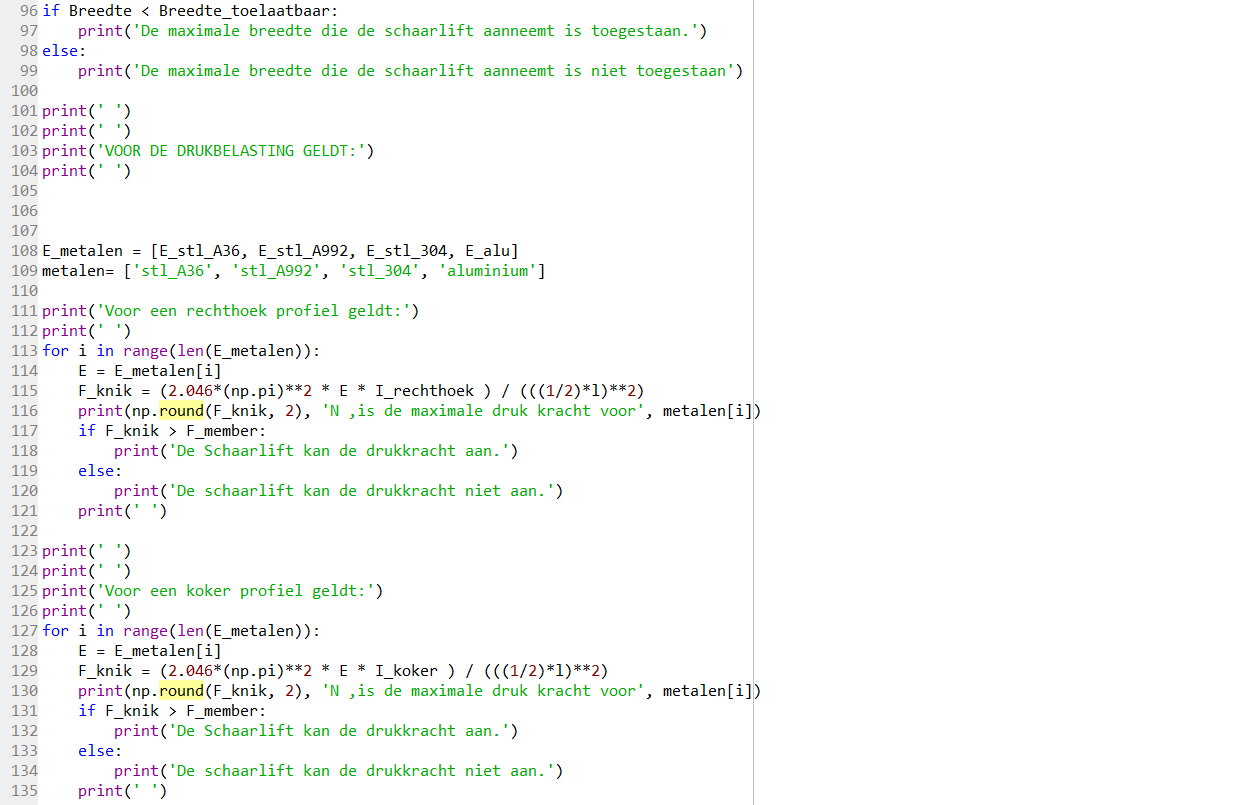
\includegraphics[width = 120mm]{06_bijlage_F/Schaarlift_script/prints2_schaarlift.PNG}
    \caption{Python script, schaarliften.}
    \label{fig:schaarliften_sript2}
\end{figure}
\vspace{\baselineskip}

\section{U-profiel aan de onderkant van de kar}
\label{se: onderkant_u-profiel}

\begin{figure}[H]
    \centering
    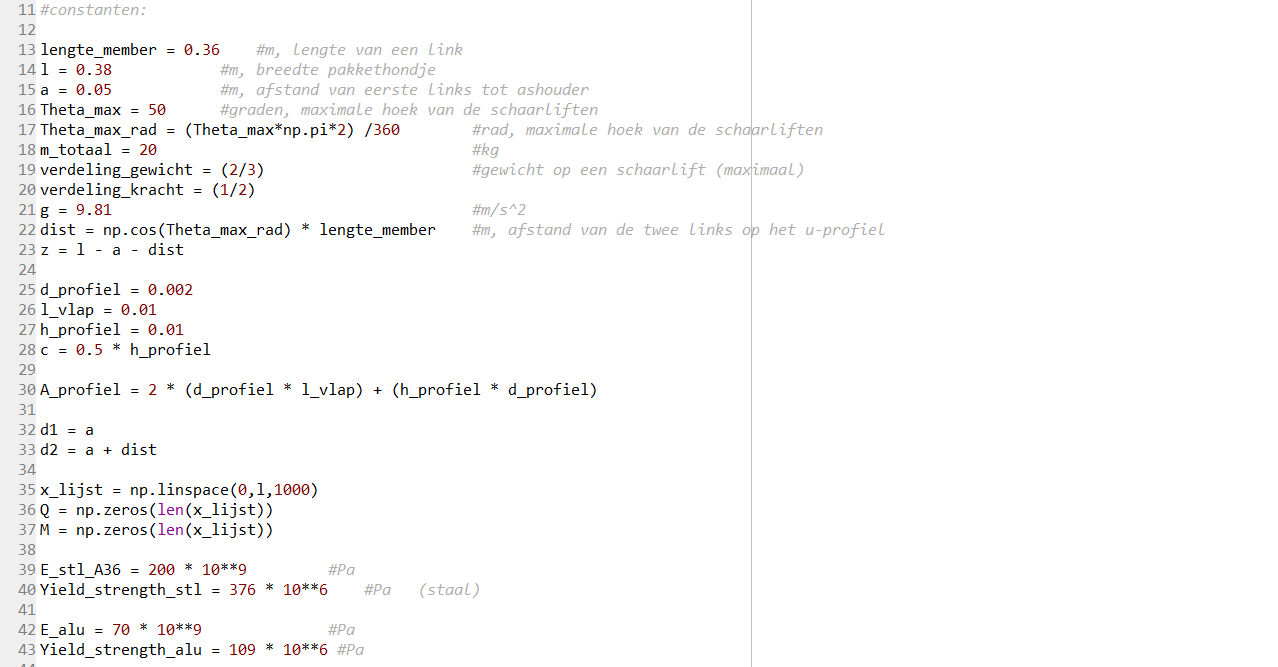
\includegraphics[width = 120mm]{06_bijlage_F/onderkant_u_profiel/constanten_onderkant.PNG}
    \caption{Python script, u-profiel.}
    \label{fig:u-profiel_constanten}
\end{figure}
\vspace{\baselineskip}

\begin{figure}[H]
    \centering
    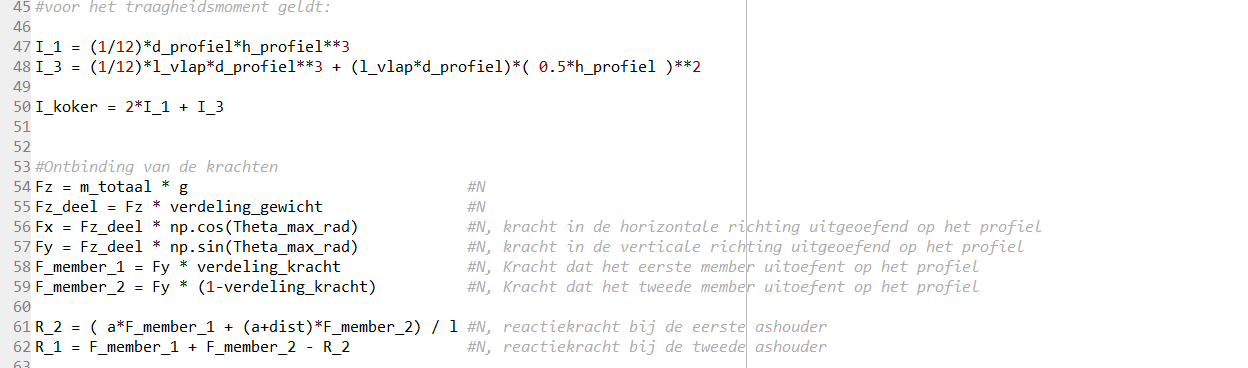
\includegraphics[width = 120mm]{06_bijlage_F/onderkant_u_profiel/krachtenanalyse_onderkant.PNG}
    \caption{Python script, u-profiel.}
    \label{fig:u-profiel_krachtenanalyse}
\end{figure}
\vspace{\baselineskip}

\begin{figure}[H]
    \centering
    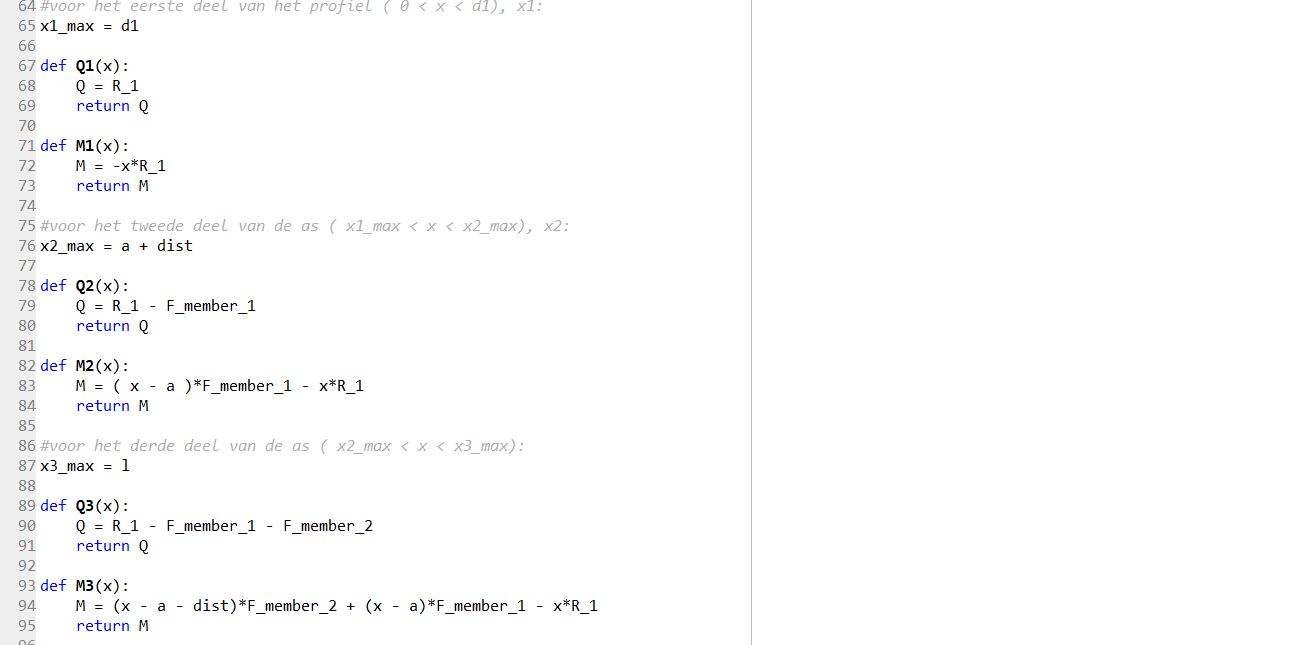
\includegraphics[width = 120mm]{06_bijlage_F/onderkant_u_profiel/formules_onderkant.PNG}
    \caption{Python script, u-profiel.}
    \label{fig:u-profiel_formules}
\end{figure}
\vspace{\baselineskip}

\begin{figure}[H]
    \centering
    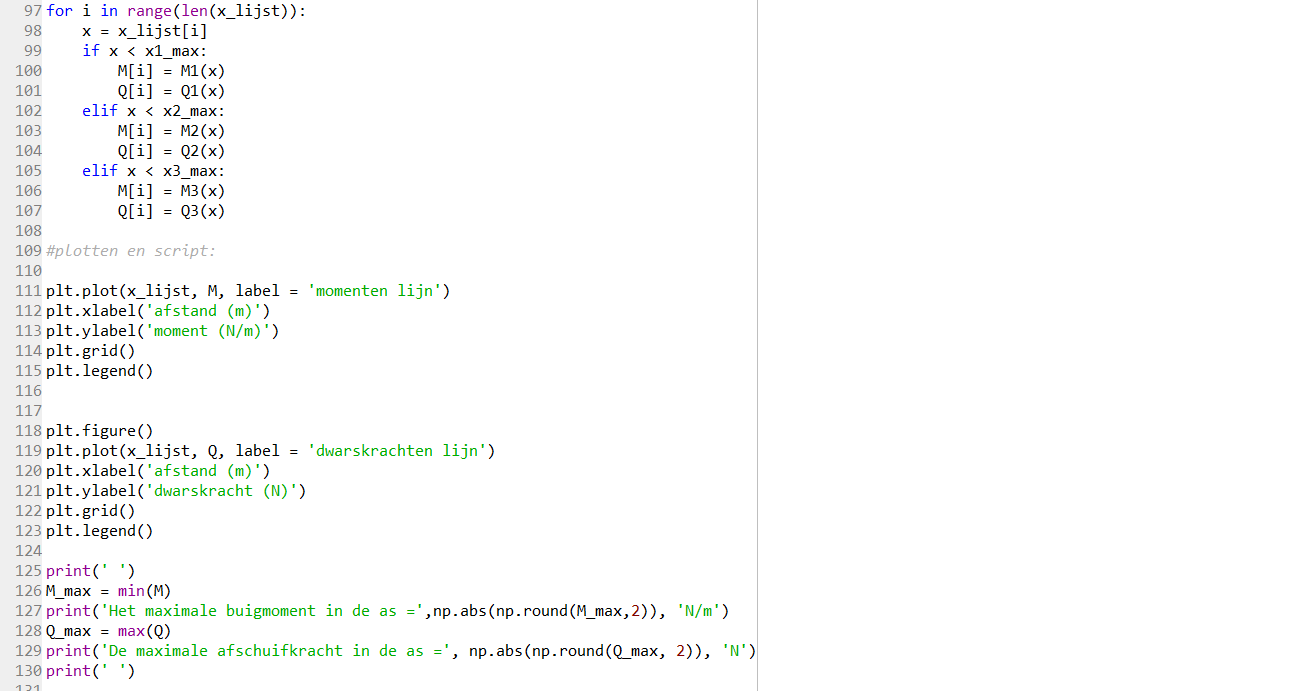
\includegraphics[width = 120mm]{06_bijlage_F/onderkant_u_profiel/forloop_onderkant.PNG}
    \caption{Python script, u-profiel.}
    \label{fig:u-profiel_forloop}
\end{figure}
\vspace{\baselineskip}

\begin{figure}[H]
    \centering
    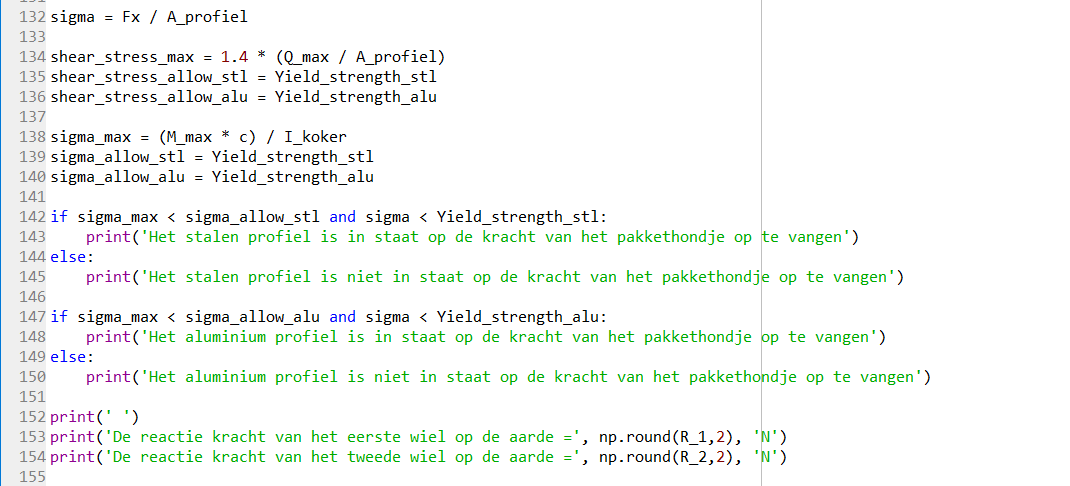
\includegraphics[width = 120mm]{06_bijlage_F/onderkant_u_profiel/print2_onderkant.PNG}
    \caption{Python script, u-profiel.}
    \label{fig:u-profiel_print}
\end{figure}
\vspace{\baselineskip}






